\documentclass{ximera}

\usepackage{todonotes}

\newcommand{\RR}{\mathbb R}
\renewcommand{\d}{\,d}
\newcommand{\dd}[2][]{\frac{d #1}{d #2}}
\renewcommand{\l}{\ell}
\newcommand{\ddx}{\frac{d}{dx}}
\newcommand{\dfn}{\textbf}
\newcommand{\eval}[1]{\bigg[ #1 \bigg]}
\renewcommand{\epsilon}{\varepsilon}
\newcommand{\p}[1]{\left(#1\right)}
\newcommand{\br}[1]{\left[#1\right]}
\newcommand{\set}[1]{\left\{#1\right\}}


\let\prelim\lim
\renewcommand{\lim}{\displaystyle\prelim}

\colorlet{textColor}{black} 
\colorlet{background}{white}
\colorlet{penColor}{blue!50!black} % Color of a curve in a plot
\colorlet{penColor2}{red!50!black}% Color of a curve in a plot
\colorlet{penColor3}{red!50!blue} % Color of a curve in a plot
\colorlet{penColor4}{green!50!black} % Color of a curve in a plot
\colorlet{penColor5}{orange!80!black} % Color of a curve in a plot
\colorlet{fill1}{blue!50!black!20} % Color of fill in a plot
\colorlet{fill2}{blue!10} % Color of fill in a plot
\colorlet{fillp}{fill1} % Color of positive area
\colorlet{filln}{red!50!black!20} % Color of negative area
\colorlet{gridColor}{gray!50} % Color of grid in a plot


\newcommand{\fullwidth}{}
\newcommand{\normalwidth}{}



%% makes a snazzy t-chart for evaluating functions
\newenvironment{tchart}{\rowcolors{2}{}{background!90!textColor}\array}{\endarray}


\author{Gregory Hartman \and Matthew Carr}
\license{Creative Commons 3.0 By-NC}
\acknowledgement{https://github.com/APEXCalculus}

\begin{document}


\begin{exercise}

\outcome{Evaluate the limit as $x$ approaches a point where there is a vertical asymptote.}
\outcome{Identify when a limit does not exist.}

\tag{limit} 
\tag{discontinuous}
\tag{vertical asymptote}

  Find 
  \[
  \lim_{x\to0} \p{\frac{x+1}{x^2+3x}}
  \begin{prompt}
  = \answer{\text{DNE}}.
  \end{prompt}
  \]
    \begin{hint}
      This function is \underline{not} continuous everywhere, but both the numerator and denominator are continuous everywhere as functions. Thus, if the limit of $\frac{x+1}{x^2+3x}$ as $x\to a$ does not exist, then the denominator $x^2+3x$ must be zero at $a$.
    \end{hint}
     \begin{hint}
    Take a look at the graph of the function
    \begin{center}
     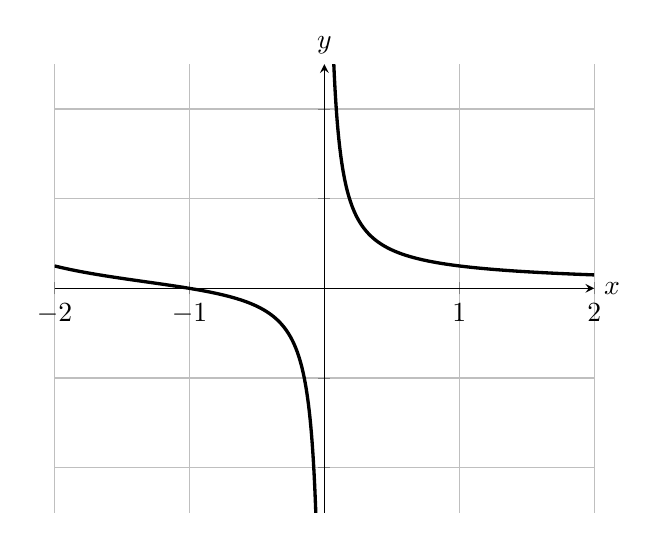
\begin{tikzpicture}
	\begin{axis}
	[ymin=-5,ymax=5, axis lines=center,xlabel=$x$,ylabel=$y$,every axis y 
	label/.style={at=(current axis.above origin),anchor=south},every axis x label/.style={at=(current axis.right of origin),anchor=west},
	domain=-2:2,
	yticklabels={},
	ymajorgrids=true,
	grid = major
	]
	\addplot[domain=-2:-1/100,very thick,smooth,samples=500]
	{(\x+1)/(\x^2+3*\x)};
	\addplot[domain=1/100:2,very thick,smooth,samples=500]
	{(\x+1)/(\x^2+3*\x)};
	\end{axis}
       \end{tikzpicture}      
      \end{center}
     Apply the limit law which says that, if both $\lim_{x\to a}f\p{x}$ and $\lim_{x\to a}g\p{x}$ exist, then, if $\lim_{x\to a}g\p{x}\ne0$, then $\lim_{x\to{a}}\frac{f\p{x}}{g\p{x}}=\frac{\lim_{x\to a}f\p{x}}{\lim_{x\to{a}}g\p{x}}$. Observe what happens around (but not at) $x=0$.
    \end{hint}
    \begin{hint}
     On the one hand, for $-3<x<0$, $x^2+3x<0$ and for $-1<x<0$, $x+1>0$; hence, for $-1<x<0$, $\frac{x+1}{x^2+3x}<0$; conversely, for $x>0$, $\frac{x+1}{x^2+3x}>0$. On the other hand, for every number $a$ satisfying $-1<a<0$ or $a>0$, the limit  $\lim_{x\to a}\p{\frac{x+1}{x^2+3x}}$ exists because both the numerator and the denominator are continuous and nonzero for all $x$ satisfying $-1<x<0$ or $x>0$. Applying several limit laws tells us that $\lim_{x\to a}\p{x+1}=\lim_{x\to a}\p{x}+\lim_{x\to a}\p{1}=a+1$ and $\lim_{x\to a}\p{x^2+3x}=\left(\lim_{x\to a}\p{x}\right)^2+3\cdot\lim_{x\to a}\p{x}=a^2+3a$. Hence, as both limits of the preceeding functions exist and $a^2+3a\ne0$ for $-1<a<0$ or $a>0$, $\lim_{x\to a}\p{\frac{x+1}{x^2+3x}}=\frac{\lim_{x\to a}\p{x+1}}{\lim_{x\to a}\p{x^2+3x}}=\frac{a+1}{a^2+3a}$.
     
     Combining these two observations with the fact that for any $a<0$, we can make the denominator arbitrarily close to $0$, while the numerator becomes arbitrarily close to $1$, we see that $\lim_{x\to0^{-}}\p{\frac{x+1}{x^2+3x}}=-\infty$. Similarly, when $a$ approaches $0$ from the right, $\lim_{x\to0^{+}}\p{\frac{x+1}{x^2+3x}}=\infty$. Since these are not equal, the limit does not exist.
     \end{hint}
\end{exercise}

\end{document}